

\tikzset{every picture/.style={line width=0.75pt}} %set default line width to 0.75pt        

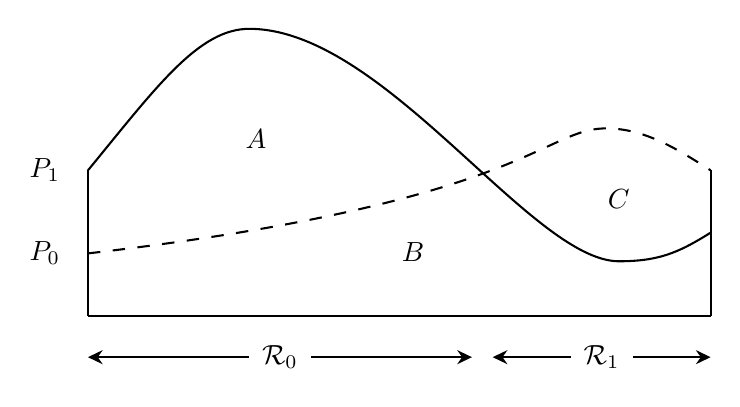
\begin{tikzpicture}[x=0.75pt,y=0.75pt,yscale=-1,xscale=1]
%uncomment if require: \path (0,178); %set diagram left start at 0, and has height of 178

%Straight Lines [id:da36257954469734544] 
\draw    (70,140) -- (370,140) ;
%Straight Lines [id:da7236983033636388] 
\draw    (70,70) -- (70,140) ;
%Straight Lines [id:da6165923641727589] 
\draw    (370,70) -- (370,140) ;
%Curve Lines [id:da901864953155475] 
\draw    (70,70) .. controls (103,29.8) and (123.36,1.75) .. (147.8,1.8) .. controls (212.68,1.94) and (282.98,112.93) .. (325.4,113.8) .. controls (344.24,113.81) and (353.8,110.2) .. (370,100) ;
%Curve Lines [id:da2681996341594639] 
\draw  [dash pattern={on 4.5pt off 4.5pt}]  (70,110) .. controls (283.4,85.4) and (289.8,48.6) .. (321,49.8) .. controls (338.6,50.2) and (354.2,59.8) .. (370,70) ;
%Straight Lines [id:da020360043822280627] 
\draw    (73,160) -- (252,160) ;
\draw [shift={(255,160)}, rotate = 180] [fill={rgb, 255:red, 0; green, 0; blue, 0 }  ][line width=0.08]  [draw opacity=0] (7.14,-3.43) -- (0,0) -- (7.14,3.43) -- (4.74,0) -- cycle    ;
\draw [shift={(70,160)}, rotate = 0] [fill={rgb, 255:red, 0; green, 0; blue, 0 }  ][line width=0.08]  [draw opacity=0] (7.14,-3.43) -- (0,0) -- (7.14,3.43) -- (4.74,0) -- cycle    ;
%Straight Lines [id:da9288058437346971] 
\draw    (268,160) -- (367,160) ;
\draw [shift={(370,160)}, rotate = 180] [fill={rgb, 255:red, 0; green, 0; blue, 0 }  ][line width=0.08]  [draw opacity=0] (7.14,-3.43) -- (0,0) -- (7.14,3.43) -- (4.74,0) -- cycle    ;
\draw [shift={(265,160)}, rotate = 0] [fill={rgb, 255:red, 0; green, 0; blue, 0 }  ][line width=0.08]  [draw opacity=0] (7.14,-3.43) -- (0,0) -- (7.14,3.43) -- (4.74,0) -- cycle    ;
%Shape: Rectangle [id:dp8000548924440445] 
\draw  [draw opacity=0][fill={rgb, 255:red, 255; green, 255; blue, 255 }  ,fill opacity=1 ] (147.5,150) -- (177.5,150) -- (177.5,170) -- (147.5,170) -- cycle ;
%Shape: Rectangle [id:dp3066289561795965] 
\draw  [draw opacity=0][fill={rgb, 255:red, 255; green, 255; blue, 255 }  ,fill opacity=1 ] (302.5,150) -- (332.5,150) -- (332.5,170) -- (302.5,170) -- cycle ;

% Text Node
\draw (151,54.8) node    {$A$};
% Text Node
\draw (226.6,109.4) node    {$B$};
% Text Node
\draw (325.8,83.8) node    {$C$};
% Text Node
\draw (58,70) node [anchor=east] [inner sep=0.75pt]    {$P_{1}$};
% Text Node
\draw (58,110) node [anchor=east] [inner sep=0.75pt]    {$P_{0}$};
% Text Node
\draw (162.5,160) node  [color={rgb, 255:red, 0; green, 0; blue, 0 }  ,opacity=1 ]  {$\mathcal{R}_{0}$};
% Text Node
\draw (317.5,160) node  [color={rgb, 255:red, 0; green, 0; blue, 0 }  ,opacity=1 ]  {$\mathcal{R}_{1}$};


\end{tikzpicture}